\chapter*{Ejercicio 9}
\section*{Ejercicio 9}

\textbf{9.} Construir las Tableaux de las siguientes proposiciones y, a partir de estas, determinar si son tautologías, contradicciones o contingentes:\\
\newline
\begin{enumerate}
\renewcommand{\theenumi}{\alph{enumi}} %Letras minúsculas 
    \item $p \rightarrow (q \lor p)$
    \item $p \rightarrow (q \land p)$
    \item $(p \land q) \leftrightarrow \neg(q \lor s)$
    \item $((p \rightarrow q)\land q) \rightarrow q$
    \item $(\neg(p \leftrightarrow q) \land (p \rightarrow q)) \rightarrow q$
    \item $((p \rightarrow q)\land (q \rightarrow \neg r)) \land r) \rightarrow (\neg p \land \neg q) $
\end{enumerate}
Para la consrucción de los tableaux debemos tener presentes las $\alpha-reglas$, $\beta-reglas$ y $\sigma-reglas$.\\
También recordemos que toda hoja qe tenga como ancestro a su negación será una rama cerrada.\\
\newline 
Con esto podemos empezar la contrucción de los tableux.\\
\newline
\textbf{Para a)}
\begin{center}
\[
\begin{array}{c}
p \rightarrow (q \lor p)\\
/ \quad \backslash\\
\neg p \quad \quad q \lor p\\
\quad \quad \quad \quad / \quad \backslash\\
\quad \quad \quad \quad q \quad p \\
\end{array}
\]
\end{center}
Ya que no podemos expandir más el árbol y ninguna rama cerró debemos probar con la negación de la proposición.
\begin{center}
\[
\begin{array}{c}
\neg(p \rightarrow (q \lor p))\\
|\\
p\\
|\\
\neg (q \lor p)\\
|\\
\neg q \\
|\\
\neg p\\
\otimes\\
\end{array}
\]
\end{center}
Se cierra ya que $p$ y $\neg p$ están en la misma rama.\\
$\therefore p \rightarrow (q \lor p)$ es tautología. \\
\newline

\textbf{Para b)}
\begin{center}
\[
\begin{array}{c}
p \rightarrow (q \land p)\\
/ \quad \backslash\\
\neg p \quad \quad q\land p\\
\quad \quad \quad  | \\
\quad \quad \quad  q \\
\quad \quad \quad  | \\
\quad \quad \quad  p \\
\end{array}
\]
\end{center}
Ya que no podemos expandir más el árbol y ninguna rama cerró debemos probar con la negación de la proposición.
\begin{center}
\[
\begin{array}{c}
\neg(p \rightarrow (q \land p))\\
/ \\
p \\
| \\
\neg(q \land p)\\
/ \quad \backslash \\
\neg q \quad \quad \neg p \\
\quad \quad \quad \otimes \\
\end{array}
\]
\end{center}
En ninguno de los casos se cierra por completo el tableux\\
$\therefore p \rightarrow (q \land p)$ es contingencia.\\
\newline

\textbf{Para c)}\\
Empezando por la eliminación de $\leftrightarrow$\\
\[
(p \land q) \leftrightarrow \neg(q \lor s)
\]
\[
(\neg(p \land q) \lor \neg (q \lor s))\land ((p \land q) \lor (q \lor s))
\]
Para formar el tableux
\begin{center}
\[
\begin{array}{c}
(\neg(p \land q) \lor \neg (q \lor s))\land ((p \land q) \lor (q \lor s))\\
| \\
\neg(p \land q) \lor \neg (q \lor s) \\
| \\
(p \land q) \lor (q \lor s) \\
/ \quad \quad \quad \quad \quad \quad \backslash \\
\neg (p \land q) \quad \quad \quad \quad \neg (q \lor s) \\
\quad / \quad \quad \quad  \backslash \quad \quad \quad \quad / \quad \quad  \backslash \\
\quad \quad \quad (p \land q) \quad (q\lor s) \quad  (p \land q) \quad (q \lor s) \\
\quad \quad / \quad \backslash \quad \quad / \quad \backslash \quad  \quad \quad | \quad \quad \quad | \\
\quad \neg p \quad \neg q \quad \neg p \quad \neg q \quad \quad \neg q \quad \quad \neg q \\
 \quad \quad   | \quad  \quad | \quad / \quad \backslash / \quad \backslash \quad \quad | \quad \quad \quad |\\
 \quad \quad p \quad \quad  p \quad q \quad s \quad q \quad s \quad \neg s \quad
 \quad \neg s \\
\quad \quad  \quad  \otimes \quad \quad | \quad \quad \quad \quad  \otimes \quad \quad | \quad \quad \quad / \quad \backslash \\
\quad \quad \quad \quad \quad \quad q \quad \quad \quad \quad \quad  \quad \quad  p \quad \quad q \quad \quad s \\
\quad \quad \quad \quad \quad \quad \quad \otimes \quad \quad \quad \quad \quad  \quad \quad  | \quad \quad \otimes \quad \quad \otimes \\
\quad \quad \quad \quad \quad \quad \quad  \quad \quad \quad \quad \quad  \quad \quad  q \quad \quad \quad  \quad \quad \\\
 \quad \quad \quad \quad \quad \quad \quad  \quad \quad \quad \quad \quad  \quad \quad  \otimes \quad \quad \quad  \quad \quad \\
\end{array}
\]
\end{center}
Puesto que no todas las ramas se cerraron probaremos con la negación de la proposición.

\begin{center}
\[
\begin{array}{c}
\neg ((\neg(p \land q) \lor \neg (q \lor s))\land ((p \land q) \lor (q \lor s)))\\
/ \quad \quad \quad \quad \quad \quad \backslash \\
\neg (\neg(p \land q) \lor \neg (q \lor s)) \quad \neg ((p \land q) \lor (q \lor s)) \\
\quad | \quad \quad \quad \quad \quad \quad \quad \quad \quad |\\
\quad p \land q \quad \quad \quad \quad \quad \quad \neg (p\land q) \\
\quad | \quad \quad \quad \quad \quad \quad \quad \quad \quad |\\
\quad q \lor s \quad \quad \quad \quad \quad \quad \neg (q \lor s) \\
\quad | \quad \quad \quad \quad \quad \quad  \quad \quad / \quad \backslash \\
\quad q \quad \quad \quad  \quad \quad  \quad \quad \neg p \quad \neg q \\
\quad /  \quad \backslash \quad \quad \quad \quad \quad  \quad \quad  | \quad \quad | \quad  \\
\quad q  \quad \quad s \quad \quad \quad \quad   \quad \quad  \neg q \quad \quad \neg q \quad  \\
\quad   \quad \quad  \quad \quad \quad \quad \quad   \quad \quad  | \quad \quad | \quad  \\
\quad   \quad \quad  \quad \quad \quad \quad \quad   \quad \quad  \neg s\quad \quad \neg s \quad  \\
\end{array}
\]
\end{center}
Puesto que tampoco se llego a una contradicción \\
$\therefore (p \land q) \leftrightarrow \neg(q \lor s)$ es contingencia.\\



\textbf{Para d)}
\begin{center}
\[
\begin{array}{c}
((p \rightarrow q)\land q) \rightarrow q\\
\quad \quad \quad \quad \quad  / \quad \backslash \\
\quad \quad \neg(p\rightarrow q)\land p \quad q \quad \quad \\
\quad \quad  | \\
\quad \neg (p \rightarrow q) \\
\quad \quad |\\
\quad \quad p \\
\quad \quad | \\
\quad \quad p \\
\quad \quad | \\
\quad \quad \neg q \\
\end{array}
\]
\end{center}
Ya que no podemos expandir más el árbol y ninguna rama cerró debemos probar con la negación de la proposición.
\begin{center}
\[
\begin{array}{c}
\neg(((p \rightarrow q)\land q) \rightarrow q)\\
| \\
(p \rightarrow q) \land p \\
|\\
\neg q \\
|\\
p \rightarrow q \\
| \\
p \\
/ \quad \backslash \\
\neg p \quad \quad q \\
\otimes \quad \quad \otimes \\
\end{array}
\]
\end{center}
Se cierra ya que la negación de $\neg p$ y $q$ se encuentran en sus respectivas ramas.\\
$\therefore ((p \rightarrow q)\land q) \rightarrow q$ es tautología.\\
\newline

\textbf{Para e)}
\[
(\neg(p \leftrightarrow q) \land (p \rightarrow q)) \rightarrow q
\]
\[
(\neg((p \rightarrow q)\land (q \rightarrow p)) \land (p \rightarrow q)) \rightarrow q
\]
\begin{center}
\[
\begin{array}{c}
(\neg((p \rightarrow q)\land (q \rightarrow p)) \land (p \rightarrow q)) \rightarrow q \\
\quad \quad \quad \quad / \quad \quad \quad \quad \quad \quad \quad \backslash \\
\neg(\neg((p \rightarrow q)\land (q \rightarrow p)) \land (p \rightarrow q))\quad \quad  q \quad \quad\\
/ \quad \quad \quad \quad \quad \quad \quad \quad\backslash \quad \quad \quad \quad\\
(p \rightarrow q)\land (q \rightarrow p) \quad  \neg (p \rightarrow q) \quad \quad \\
| \quad \quad  \quad \quad  \quad \quad \quad \quad | \\
(p \rightarrow q) \quad \quad  \quad \quad  \quad \quad  p \\
| \quad \quad  \quad \quad  \quad \quad \quad \quad | \\
(q \rightarrow p) \quad \quad  \quad \quad  \quad \quad  \neg q \\
/ \quad \quad \backslash \quad \quad  \quad \quad \quad \quad \quad  \\
\neg p \quad \quad q \quad \quad  \quad \quad \quad \quad \quad  \\
/ \quad \backslash \quad / \quad \backslash \quad  \quad \quad \quad \quad \quad  \\
\neg q \quad p \quad \neg q \quad p \quad  \quad \quad \quad \quad \quad  \\
\quad  \quad \otimes  \quad \otimes  \quad  \quad  \quad \quad \quad \quad \quad  \\

\end{array}
\]
\end{center}
Vemos que hay ramas que cierran y también ramas que no se cierran\\
$\therefore (\neg(p \leftrightarrow q) \land (p \rightarrow q)) \rightarrow q$ es contingencia.\\

\textbf{Para f)}
\begin{center}
\[
\begin{array}{c}
(((p \rightarrow q)\land (q \rightarrow \neg r)) \land r) \rightarrow (\neg p \land \neg q) \\
\quad \quad \quad / \quad \quad \quad \quad \quad \backslash \\
\quad \neg (((p \rightarrow q)\land (q \rightarrow \neg r))\land r)  \quad \quad (\neg p \land \neg q)\\
\quad \quad \quad \quad/ \quad \quad \quad \quad \quad  \backslash \quad \quad \quad \quad \quad \quad |\\
\neg ((p \rightarrow q)\land (q \rightarrow \neg r))\quad \neg r  \quad \quad \quad \quad \neg p\\
\quad \quad/ \quad \quad \quad \quad \quad  \backslash \quad \quad \quad \quad \quad \quad \quad |\\
\neg (p \rightarrow q) \quad \quad \neg (q \rightarrow \neg r) \quad  \quad \quad \quad  \quad \neg q \\
\quad \quad |\quad \quad \quad \quad \quad | \quad \quad \quad \quad \quad \quad \quad \quad \\
\quad \quad p\quad \quad \quad \quad \quad q \quad \quad \quad \quad \quad \quad \quad \quad \\
\quad \quad |\quad \quad \quad \quad \quad | \quad \quad \quad \quad \quad \quad \quad \quad \\
\quad \quad \neg q \quad \quad \quad \quad \quad \neg(\neg r) \quad \quad \quad \quad \quad \quad \quad \quad \\
\quad \quad \quad  \quad \quad \quad \quad \quad  r \quad \quad \quad \quad \quad \quad \quad \quad \\

\end{array}
\]
\end{center}

Puesto que no tiene ramas que cierren debemos probar con la negación de la proposición.

\begin{center}
    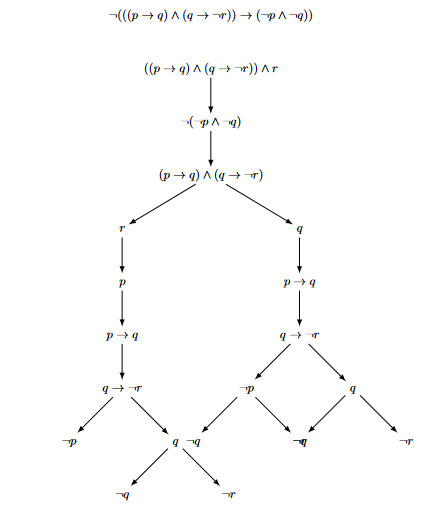
\includegraphics[height = 0.25\textheight]{recursos/imagen1.png}\par
\end{center}


Puesto que en la negación de la proposición se genera una contradición 
$\therefore (((p \rightarrow q)\land (q \rightarrow \neg r)) \land r) \rightarrow (\neg p \land \neg q) $ es tautología.\\


